\identify{Identify the Challenge \& Set Goals: MoGo Mechanism V1.1 (November 18, 2024)}
\info{Caleb Bachmeier}{MoGo Mechanism V1.1}{November 18, 2024}
\chapterauthor{Caleb Bachmeier}
\textbf{Goal}: We will identify an objective for our robot so that we can address it and build an effective solution
\section*{Problem Statement}
It became apparent after North Dakota Signature Event that the team would benefit greatly from a mechanism that would guide a Mobile Goal onto our Clamp.
\section*{Solution Requirements}
\begin{itemize}
    \item Complete before our tournament on November 23, in Harrisburg, South Dakota
\end{itemize}
\section*{Solution Goals}
\begin{itemize}
    \item The team does not want to change too much of the robot, especially this close to the next tournament.
\end{itemize}
\brainstorm{Brainstorm \& Diagram: MoGo Mechanism V1.1 (November 18, 2024)}
\info{Caleb Bachmeier}{MoGo Mechanism V1.1}{November 18, 2024}
\chapterauthor{Caleb Bachmeier}
\section*{Possible Solutions}
Some solutions the team can implement include:
\begin{itemize}
	\item Add stoppers inside the robot so that the Mobile Goal would stop at the perfect spot.
	\item Increase the size of the "clamp" part of our Clamp and add more \textit{Rubber Bumpers} (SKU: 276-7499) \vex. Shown in Figure \ref{fig:2stoppers}
\end{itemize}
\begin{figure}[H]
	\centering
	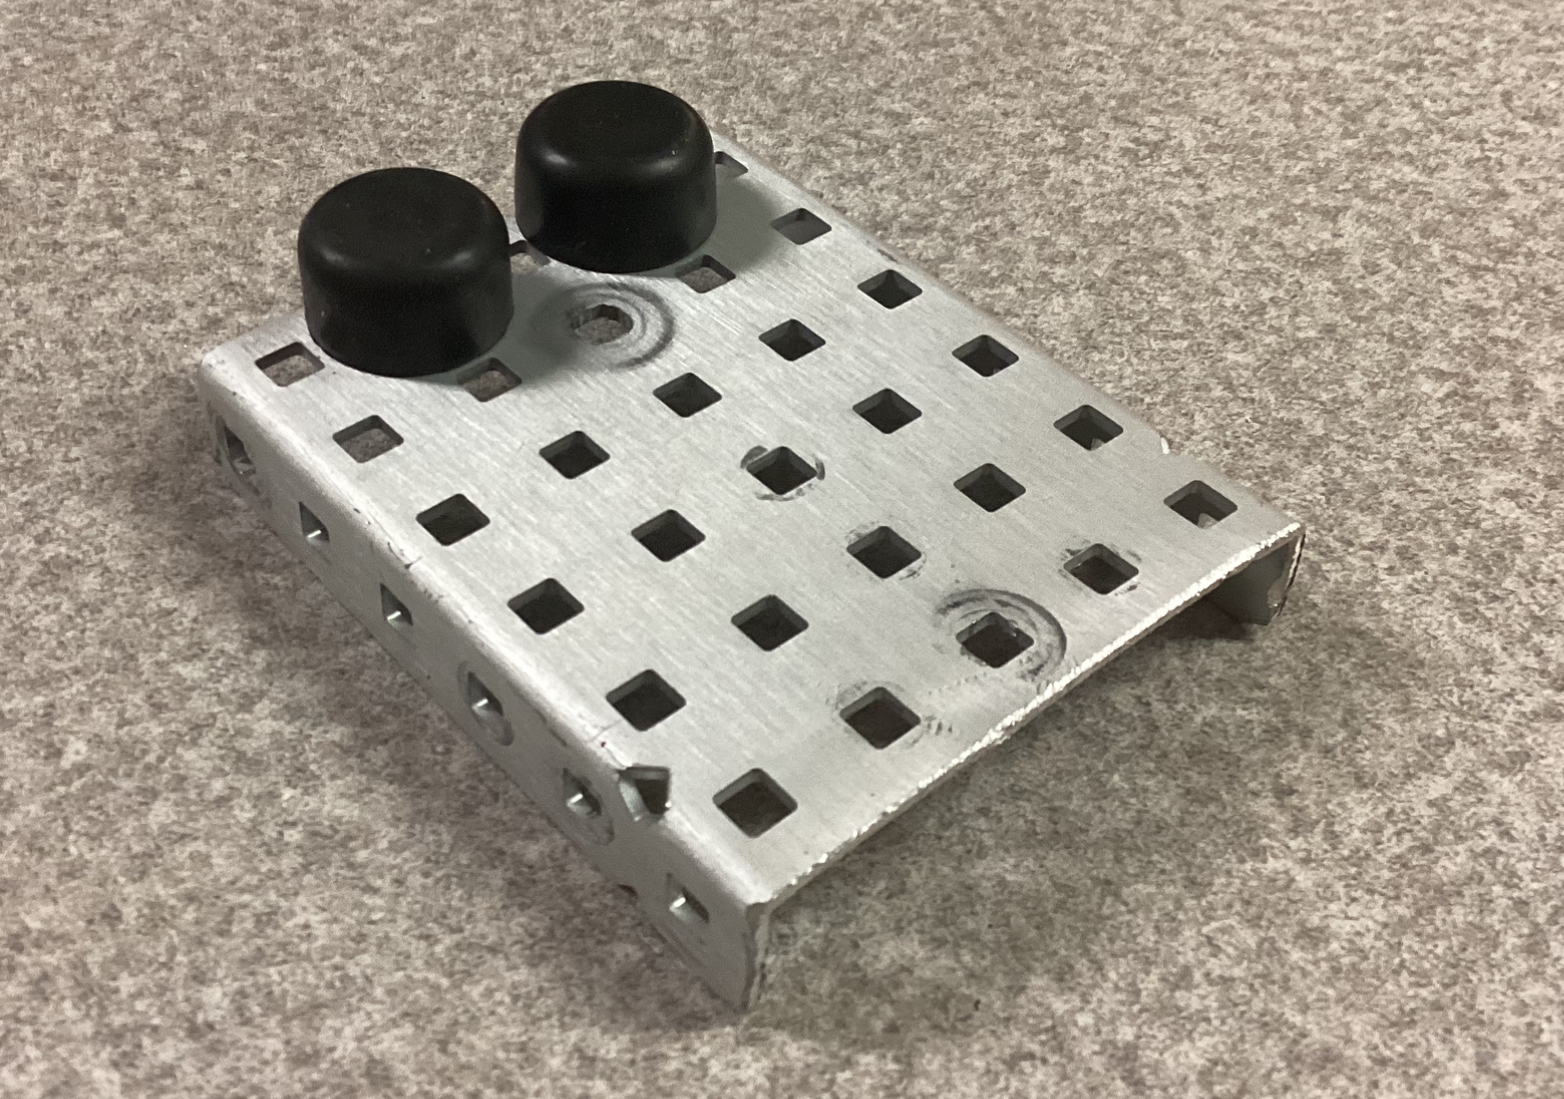
\includegraphics[width=0.5\linewidth]{images/Two Stopper.jpeg}
	\caption{Larger Clamp}
	\label{fig:2stoppers}
\end{figure}
\solution{Choose a Solution: MoGo Mechanism V1.1 (November 18, 2024)}
\info{Caleb Bachmeier}{MoGo Mechanism V1.1}{November 18, 2024}
\chapterauthor{Caleb Bachmeier}
\section*{Choose a Solution}
\renewcommand{\arraystretch}{1.85} % Change this value as needed
\begin{table}[htb!]
\centering
\begin{tabular}{|>{\centering\arraybackslash}m{1.85cm}|>{\centering\arraybackslash}m{1.85cm}|>{\centering\arraybackslash}m{1.85cm}|>{\centering\arraybackslash}m{1.85cm}|>{\centering\arraybackslash}m{1.85cm}|>{\centering\arraybackslash}m{1.85cm}|>{\centering\arraybackslash}m{1.85cm}|}
\hline
\textbf{Scale 1 - 10} & \textbf{Complexity} & \textbf{Size} & \textbf{Speed} & \textbf{Redesign Necessary?} & \textbf{Total}  \tabularnewline
\hline
Weight & x1 & x3 & x1 & x3 & \tabularnewline
\hline
Larger Clamp & 10 & 6 & 10 & 9 & 67 \tabularnewline
\hline
Stopper & 8 & 10 & 10 & 9 & 77 \tabularnewline
\hline
\end{tabular}
\caption{MoGo V1.1 Decision Matrix}
\label{tab:MoGoV1.1}
\end{table}
\renewcommand{\arraystretch}{1.85} % Reset to default
According to our point totals, it seems we will be making a stopper mechanism that with fit the Mobile Goal into the Clamp.
\section*{Make a Plan}
To build this stopper, we used High Strength Shaft Collars (SKU: 276-7580)  Figure: \ref{fig:HS-Collar} \vex 
\begin{figure}
    \centering
    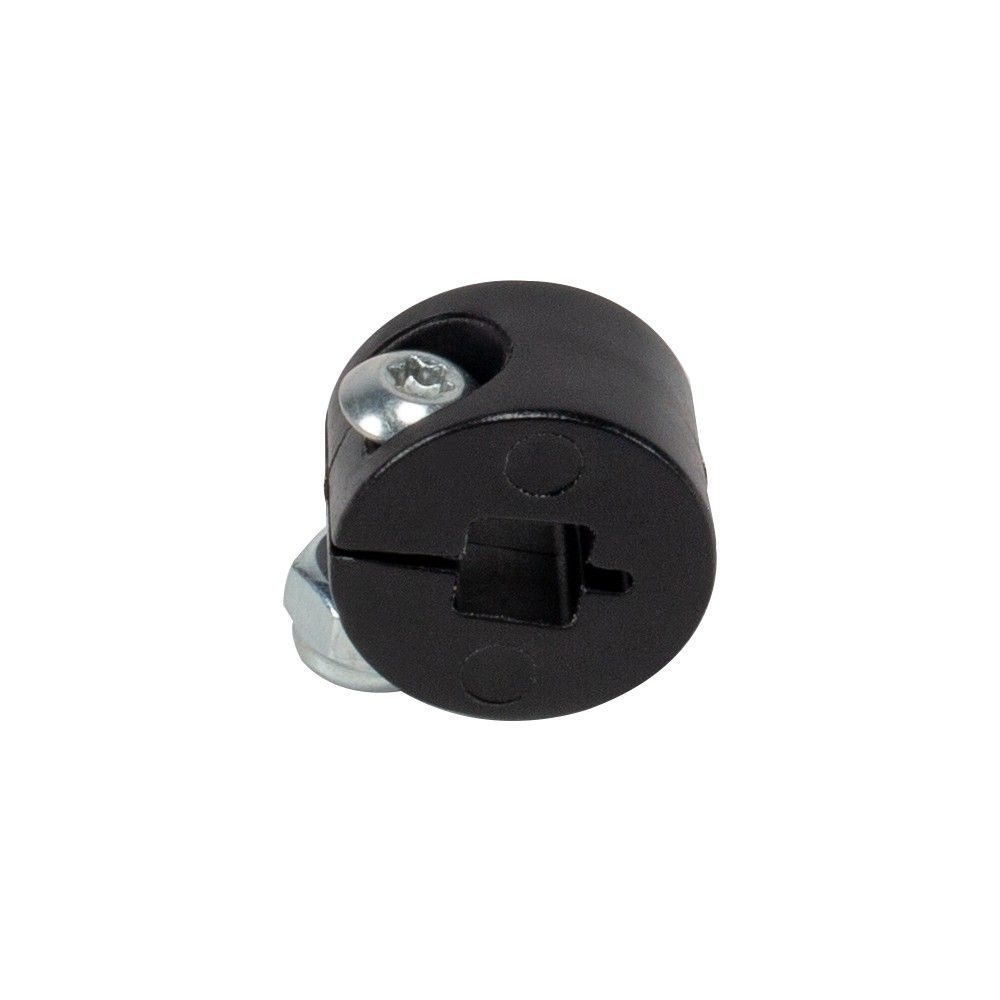
\includegraphics[width=0.3\linewidth]{images/HS Shaft Collar.jpg}
    \caption{High Strength Shaft Collar}
    \label{fig:HS-Collar}
\end{figure}
\build{Build \& Program: MoGo Mechanism V1.1 (November 18, 2024)}
\info{Caleb Bachmeier}{MoGo Mechanism V1.1}{November 18, 2024}
\chapterauthor{Caleb Bachmeier}
\section*{Building}
Building the stopper system was extremely simple. All we had to do is take a High Strength axle and attach three High Strength Shaft Collars to them. We then connected them to a C-Channel on the drivetrain, we placed them eight spaces apart (See Figure~\ref{fig:stoppers-v1.1}). This was a very simple to build.

\begin{figure}[H]
    \centering
    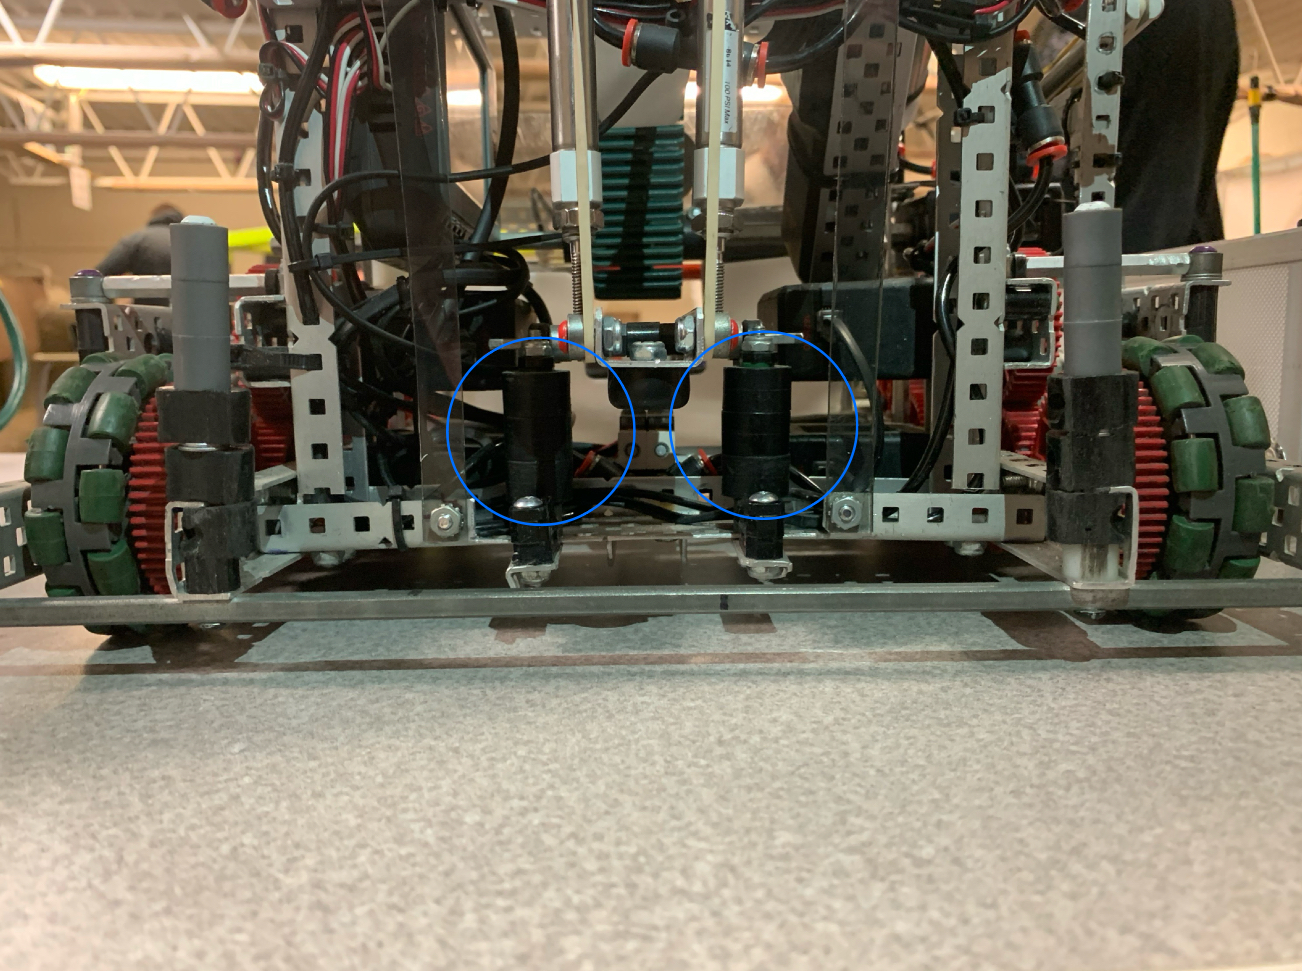
\includegraphics[width=0.5\linewidth]{images/Stoppers MoGoV1.1.jpeg}
    \caption{Built Solution}
    \label{fig:stoppers-v1.1}
\end{figure}
\test{Test the Solution: MoGo Mechanism V1.1 (November 18, 2024)}
\info{Caleb Bachmeier}{MoGo Mechanism V1.1}{November 18, 2024}
\chapterauthor{Caleb Bachmeier}
\section*{Test the Solution}
This solution was also very easy to test. We simply picked up a Mobile Goal with the Clamp, and it work as it did before. Then we tried to force the Mobile Goal into the Clamp, and it stopped in the perfect spot! This solution is a successes, and we are very happy to complete this before our tournament in Harrisbrg, South Dakota.
